\documentclass{chi-ext}
% Please be sure that you have the dependencies (i.e., additional LaTeX packages) to compile this example.
% See http://personales.upv.es/luileito/chiext/

%% EXAMPLE BEGIN -- HOW TO OVERRIDE THE DEFAULT COPYRIGHT STRIP -- (July 22, 2013 - Paul Baumann)
% \copyrightinfo{Permission to make digital or hard copies of all or part of this work for personal or classroom use is granted without fee provided that copies are not made or distributed for profit or commercial advantage and that copies bear this notice and the full citation on the first page. Copyrights for components of this work owned by others than ACM must be honored. Abstracting with credit is permitted. To copy otherwise, or republish, to post on servers or to redistribute to lists, requires prior specific permission and/or a fee. Request permissions from permissions@acm.org. \\
% {\emph{CHI'14}}, April 26--May 1, 2014, Toronto, Canada. \\
% Copyright \copyright~2014 ACM ISBN/14/04...\$15.00. \\
% DOI string from ACM form confirmation}
%% EXAMPLE END -- HOW TO OVERRIDE THE DEFAULT COPYRIGHT STRIP -- (July 22, 2013 - Paul Baumann)
\copyrightinfo{Permission to make digital or hard copies of part or all of this work for personal or classroom use is granted without fee provided that copies are not made or distributed for profit or commercial advantage and that copies bear this notice and the full citation on the first page. Copyrights for third-party components of this work must be honored. For all other uses, contact the Owner/Author. \\
Copyright is held by the owner/author(s). \\
{\emph{L@S 2015}}, Mar 14-18, 2015, Vancouver, BC, Canada \\
ACM 978-1-4503-3411-2/15/03. \\
http://dx.doi.org/10.1145/2724660.2728676}

\title{Game Theory Based Peer Grading Mechanisms For MOOCs}

\numberofauthors{5}
% Notice how author names are alternately typesetted to appear ordered in 2-column format;
% i.e., the first 4 autors on the first column and the other 4 auhors on the second column.
% Actually, it's up to you to strictly adhere to this author notation.
\author{
  \alignauthor{
    \textbf{William Wu}\\
    \affaddr{Acton Boxborough Regional High School}\\
    \affaddr{36 Charter Rd}\\
    \affaddr{Acton, MA 01720, USA}\\
    \email{willy.vvu@gmail.com}
  }\alignauthor{
    \textbf{Christos Tzamos}\\
    \affaddr{Massachusetts Institute of Technology}\\
    \affaddr{77 Massachusetts Avenue}\\
    \affaddr{Cambridge, MA 02139}\\
    \email{ctzamos@gmail.com}
  }
  \vfil
  \alignauthor{
    \textbf{Constantinos Daskalakis}\\
    \affaddr{Massachusetts Institute of Technology}\\
    \affaddr{77 Massachusetts Avenue}\\
    \affaddr{Cambridge, MA 02139}\\
    \email{costis@csail.mit.edu}
  }\alignauthor{
    \textbf{Matthew Weinberg}\\
    \affaddr{Massachusetts Institute of Technology}\\
    \affaddr{77 Massachusetts Avenue}\\
    \affaddr{Cambridge, MA 02139}\\
    \email{smweinberg@csail.mit.edu}
  }
  \vfil
  \alignauthor{
    \textbf{Nicolaas Kaashoek}\\
    \affaddr{Lexington High School}\\
    \affaddr{251 Waltham Street}\\
    \affaddr{Lexington, MA 02421, USA}\\
    \email{nick.kaashoek@gmail.com}
  }
}

% Paper metadata (use plain text, for PDF inclusion and later re-using, if desired)
\def\plaintitle{Game Theory based Peer Grading Mechanisms for MOOCs}
\def\plainauthor{William Wu}
\def\plainkeywords{MOOC, game theory, mechanism design, peer grading, learning at scale}
\def\plaingeneralterms{Game Theory, Mechanism Design, Peer Grading}

\hypersetup{
  % Your metadata go here
  pdftitle={\plaintitle},
  pdfauthor={\plainauthor},  
  pdfkeywords={\plainkeywords},
  pdfsubject={\plaingeneralterms},
  % Quick access to color overriding:
  %citecolor=black,
  %linkcolor=black,
  %menucolor=black,
  %urlcolor=black,
}

\usepackage{graphicx}   % for EPS use the graphics package instead
\usepackage{balance}    % useful for balancing the last columns
\usepackage{bibspacing} % save vertical space in references

\usepackage{epstopdf}

\begin{document}

\maketitle

\begin{abstract}
An efficient peer grading mechanism is proposed for grading the multitude of assignments in online courses. This novel approach is based on game theory and mechanism design. A set of assumptions and a mathematical model is ratified to simulate the dominant strategy behavior of students in a given mechanism. A benchmark function accounting for grade accuracy and workload is established to quantitatively compare effectiveness and scalability of various mechanisms. After multiple iterations of mechanisms under increasingly realistic assumptions, three are proposed: Calibration, Improved Calibration, and Deduction. The Calibration mechanism performs as predicted by game theory when tested in an online crowd-sourced experiment, but fails when students are assumed to communicate. The Improved Calibration mechanism addresses this assumption, but at the cost of more effort spent grading. The Deduction mechanism performs relatively well in the benchmark, outperforming the Calibration, Improved Calibration, traditional automated, and traditional peer grading systems. The mathematical model and benchmark opens the way for future derivative works to be performed and compared.
\end{abstract}

\keywords{Massive Open Online Courses; MOOC; game theory; mechanism design; peer grading; learning at scale;}

\category{K.3.m.}{Computers and Education}{Miscellaneous}. \\
See: \url{http://www.acm.org/about/class/1998/} 
for help using the ACM Classification system.

\section{Introduction}
Over the past few years, there has been a tremendous increase in the popularity of MOOCs (Massive Open Online Courses) and their importance to education as a whole. Popular MOOC systems such as Coursera or EdX are well funded, which explains their rapid growth: 60 million dollars were invested in EdX when it started in May of 2012~\cite{canMOOCsreducecc}. The main importance of MOOCs is their ability to educate massive numbers of students worldwide~\cite{makingsenseofMOOCs}: by the end of 2012, 1.7 million students had attended a course through Coursera~\cite{swotanalysisofMOOCs}. This leads to high student-professor ratios, reaching 150,000:1 in some courses.

High student-professor ratios lead to problems for professors, who are simply unable to grade hundreds of thousands of submissions. Currently, two types of solutions are used to remedy the problem: automated grading and peer grading~\cite{edxsoftware}. Automated grading relies on machines, which can only check certain types of answers (i.e. multiple choice), severely limiting the depth of the questions asked~\cite{rightandwrongMOOCs}. Even though automated grading for written essays is an active area of research with much recent progress, the quality and accuracy of such systems is under heavy debate~\cite{automatedsystemssuck}. Students who know the machine's grading criteria can fool the system~\cite{robogradingproblems}, yielding inconsistent grades. On the other hand, peer grading can grade any type of question. However, such systems can easily be ``hacked'' by the students~\cite{makingsenseofMOOCs}. Additionally, lack of feedback from peer grading is an area of complaint in systems such as Coursera~\cite{howaccurateispeergrading}. These limitations render the students unable to effectively evaluate mastery of course material. 

We propose several peer grading mechanisms based on game theory and our student model - a set of assumptions we believe students abide by. We also create a benchmark to compare between our and existing mechanisms. Although a theoretical model cannot predict exactly what will happen in practice, game theory and mechanism design have a history of generally determining mechanisms that work in practice from ones that do not~\cite{AGTbook}. Mechanisms that do not follow game theoretic constraints may work in the short-term, but they will be exploited if possible in the long term~\cite{boycottfinal}.

\section{Model and Assumptions}
\label{sec:modelandassumptions}
Our student model consists of assumptions we believed students abide by, as follows:
\begin{enumerate}
\item Let H be a function of a student's grade, returning a student's happiness, such that a grade of zero yields zero happiness ($H(0)=0$). \newline \textit{Happiness is an arbitrary numerical unit.}
\item Students want to maximize their happiness.
\item Grading an assignment costs 1 (one) happiness.
\item Happiness is not affected by external factors, such as the grades of peers.
\item Students can communicate with their peers.
\item Students are not perfect graders.
\item There is no such thing as partial-grading. Students either grade or do not grade.
\item Students can report their level of uncertainty (U) when they grade.
\item More effort spent in grading lowers uncertainty.
\item The chance of a student-assigned grade G being N off from the actual grade is proportional to U.
\end{enumerate}

With a student model in place, it is now possible to simulate student behavior with game theory.

\section{Benchmark}
In order to eventually determine the effectiveness of various mechanisms, as well as to compare mechanisms, we created a numerical benchmark (objective function) where a lower score is better. The score is computed by adding the highest possible error in student grading to the most work done by any person. Mathematically:

$\max_{i \ge 1} \{|H(g_i)-H(o_i)|\} + \max_{i \ge 1} \{w_i\}$

where $w_i$ is the work done (assignments graded) by the $i$th person, $g_i$ is the grade given by student grader on the $i$th assignment, and $o_i$ is the accurate ``objective'' grade that would have been given by the professor on the $i$th assignment. $H$ is the happiness function defined in the \textit{Models and Assumptions}~section.

\section{Mechanisms}
\subsection{Calibration Mechanism}

The Calibration mechanism, described visually in Figure~\ref{fig:calibration},achieves a low benchmark score of 4, consisting of a 2 in max work done and 2 in max error in grade.

\begin{figure}
  \centering
  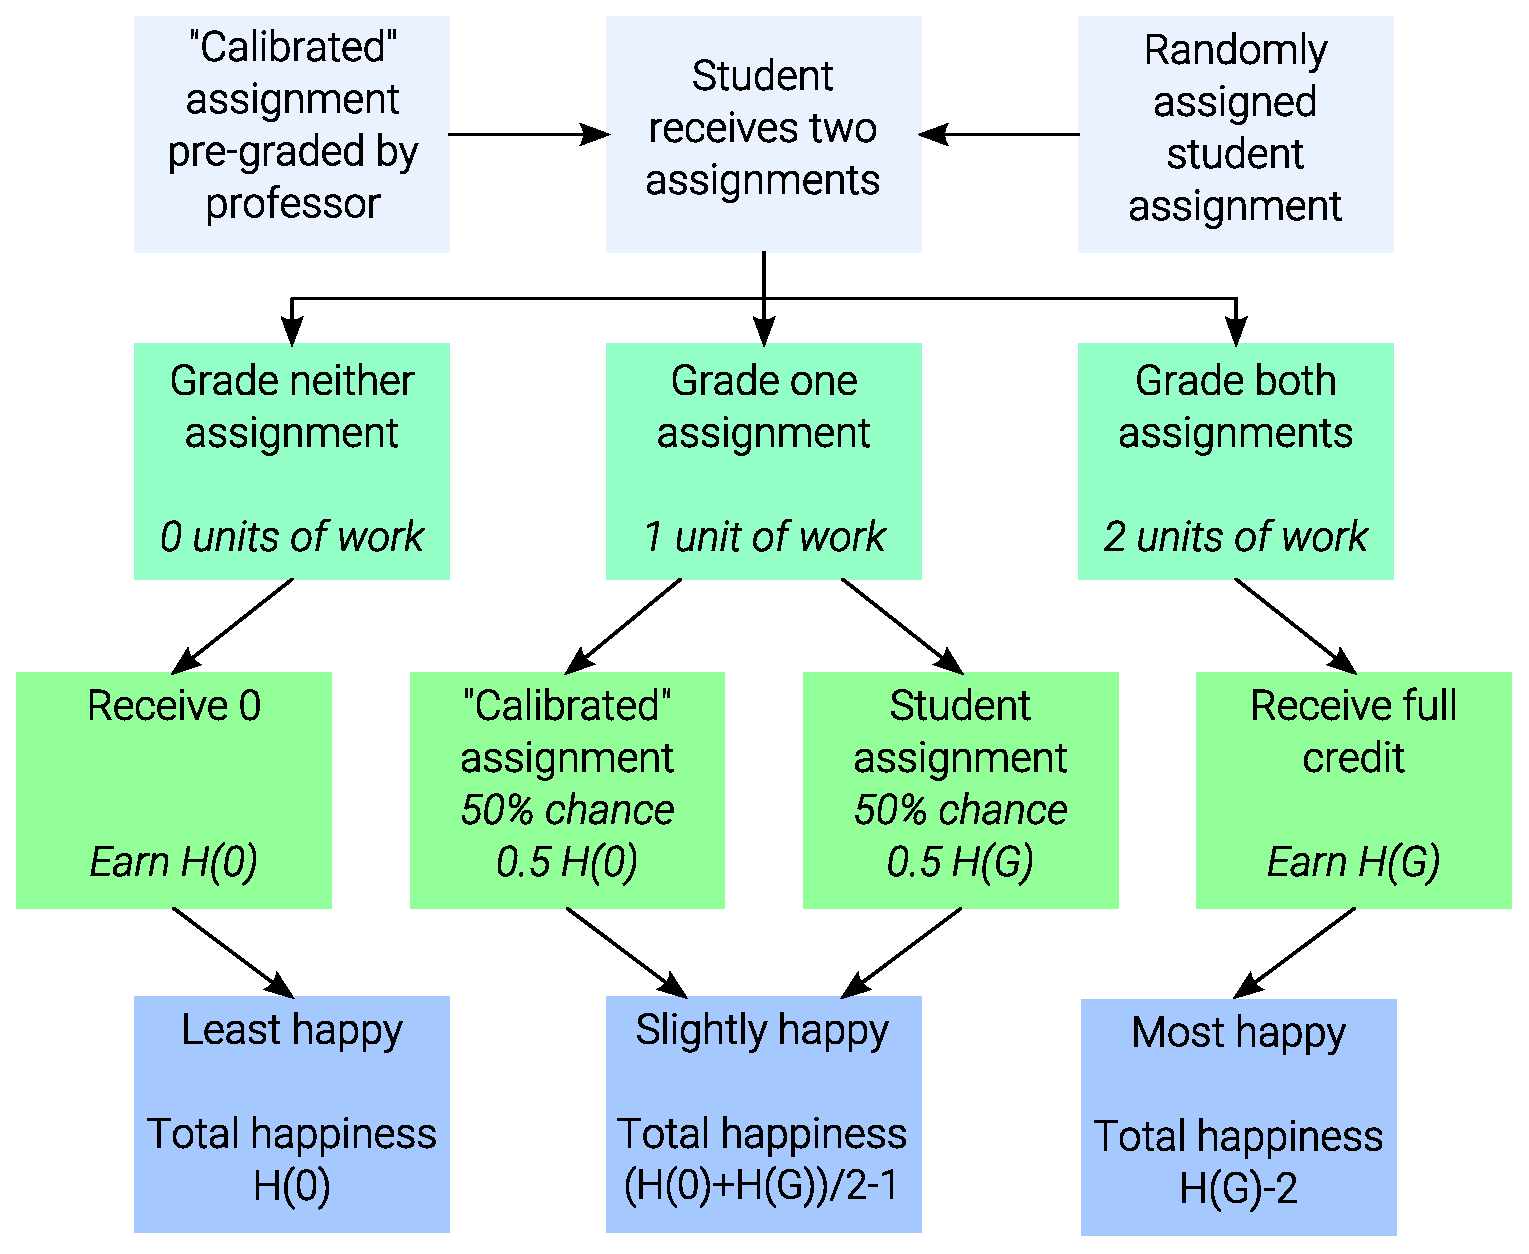
\includegraphics[width=\linewidth]{Calibration-Flowchart.eps}
  \caption{A flowchart of the Calibration Mechanism from the student perspective.}
  \label{fig:calibration}
\end{figure}

We tested and verified the Calibration mechanism through an anonymous crowd-sourced experiment. We wrote a program that presented participants with two sets of randomly generated orange and blue colored objects. Each set represented an assignment, and ``grading'' an assignment involved counting the number of orange objects in each set. After observing the set for a randomly chosen amount of time, participants were asked to input the number of orange objects they thought they saw in each set. Initially unknown to the participant, one set is ``calibrated'' and will be used to reward the participant based on the accuracy of the grading. This reward, awarded for accurately grading the Calibrated set, is synonymous to the punishment administered by the professor upon improperly grading the Calibrated set.

\begin{figure}
  \centering
  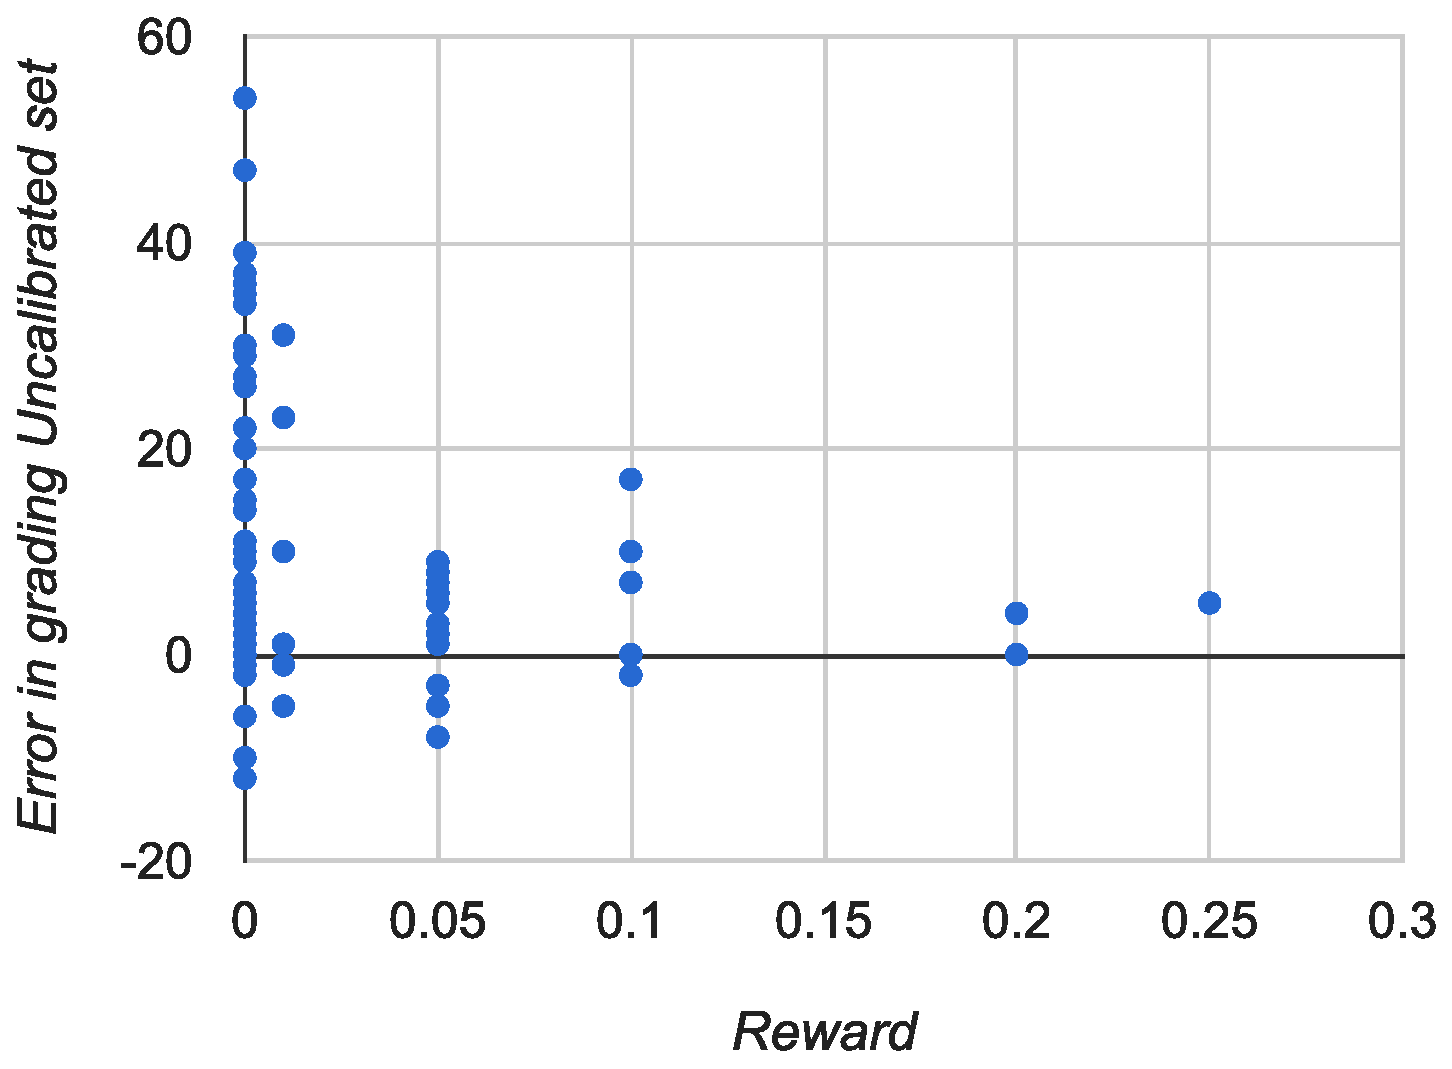
\includegraphics[width=\linewidth]{Reward-Error-Graph.eps}
  \caption{Uncalibrated Error vs Reward}
  \label{fig:reward-error}
\end{figure}

The results of this experiment can be seen in Figure~\ref{fig:reward-error}, where grading error is plotted against relative magnitude of reward. This shows that a higher reward correlates to lower error. As the reward is administered based on the grader's performance on the Calibrated set, the correlation implies that the graders who perform well on the Calibrated set also perform well on the non-calibrated set. This verifies that the Calibration mechanism indeed works.

\subsection{Improved Calibration Mechanism}
Originally designed with the assumption that students cannot communicate, the Calibration mechanism quickly breaks when student conspire to reveal the calibrated assignment to circumvent grading. The Improved Calibration mechanism mitigates this issue by introducing multiple calibrated papers at the expense of more work, raising the objective score. However, since the work created by this mechanism does not scale well with class size, the Deduction mechanism was developed.

\subsection{Deduction Mechanism}

The Deduction mechanism (Figure~\ref{fig:deduction}) achieves a very low benchmark score of 2, with 2 in max work done and a 0 in max error in grade. Incapable graders will raise the benchmark score, as they issue refutations that add work to the professor.

\begin{figure}
  \centering
  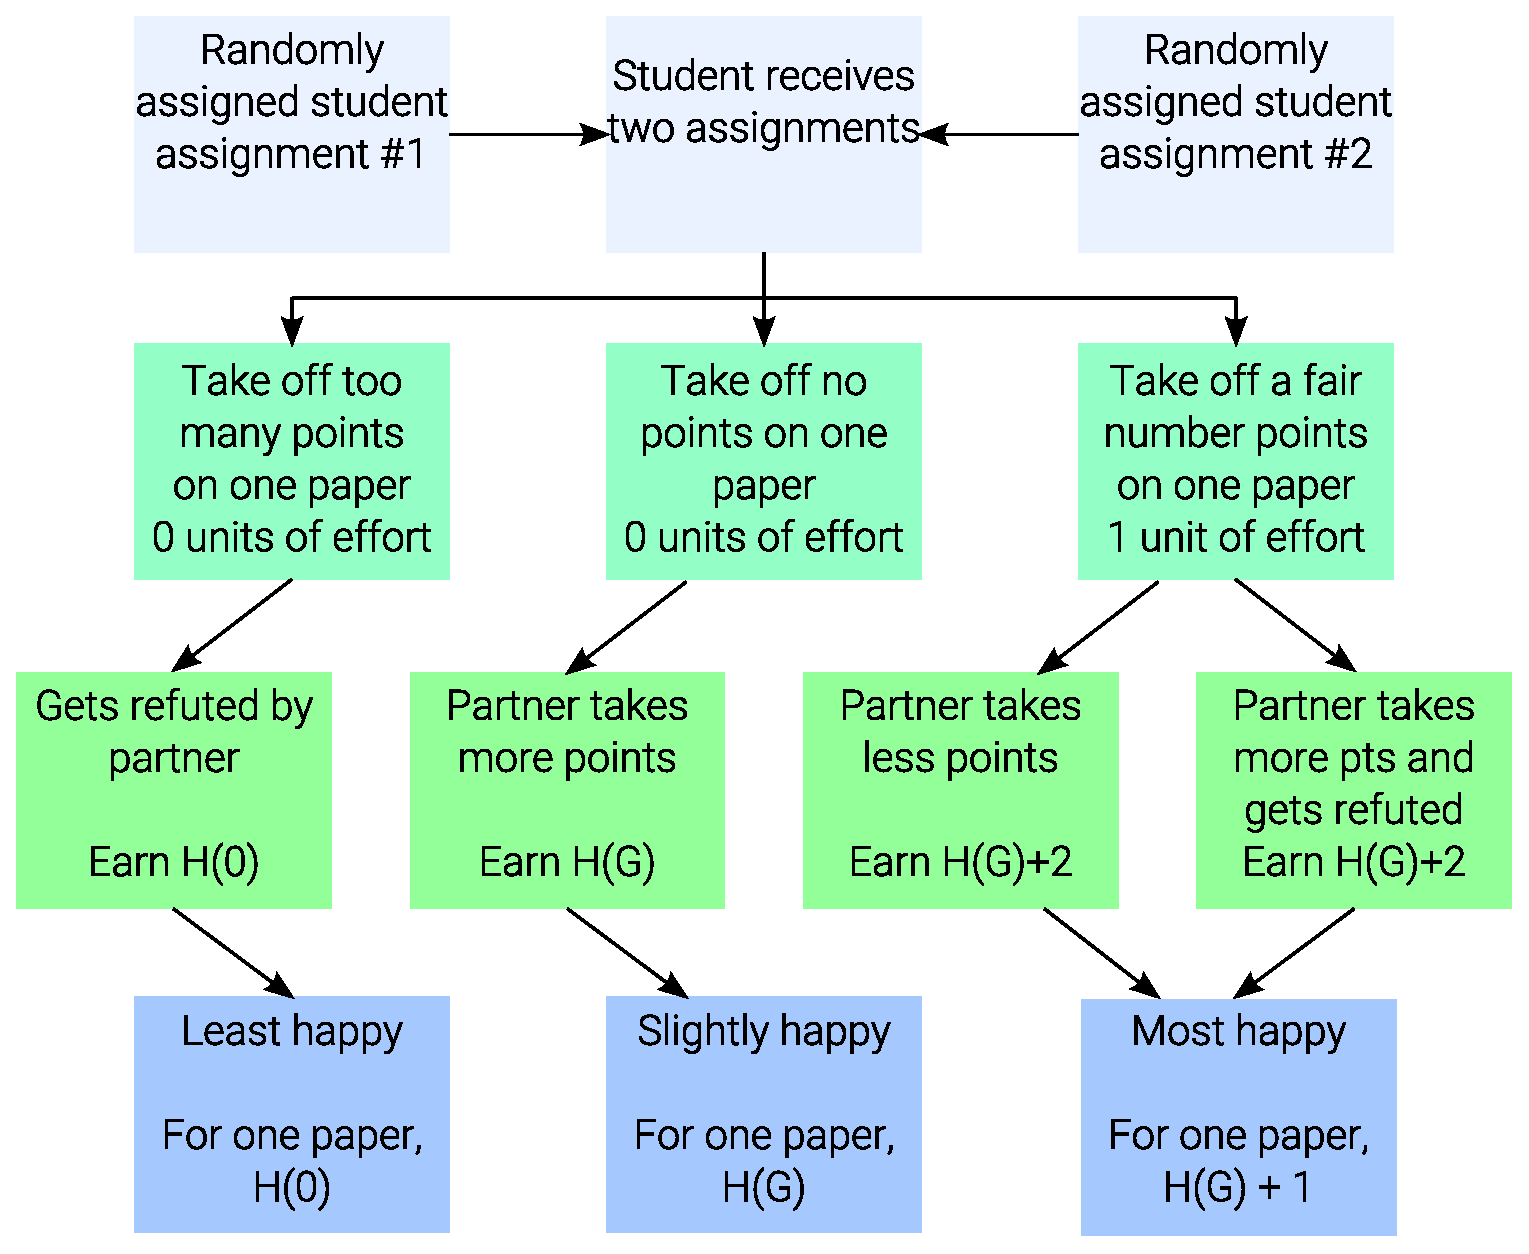
\includegraphics[width=\linewidth]{Deduction-Flowchart.eps}
  \caption{A flowchart of the Deduction Mechanism from the student perspective.}
  \label{fig:deduction}
\end{figure}

\section{Results}
The comparison of existing solutions and those proposed in this work can be seen in Figure~\ref{fig:comparison}. Each mechanism will be explained below.

Traditional Professor Grading involves one professor grading all assignments. In an online class of 1000 students, this method is extremely inefficient.

In Traditional Peer Grading, each student grades another's assignment without any supervision. However, as in this mechanism, the objective score is high due to the potential error caused by lack of motivation to grade properly.

% TODO: Add references to computer grading
Although without requiring effort from either professor or student, Traditional Automated Grading of open-ended responses are still under heavy research. Current solutions are quite preliminary, though can arrive at a grade within approximately 25 percent~\cite{automatedsystemssuck}.

The Calibration Mechanism requires one calibrated paper from the professor and two papers graded by each student. The objective score is raised to 4 instead of 2 because students are incentivized by increasing their grade, thus sacrificing accuracy.

The Improved Calibration Mechanism requires each student to grade a subset of the other student's assignments, and the teacher to grade another subset. This mechanism addresses the flaw in the Calibration Mechanism that occurs when students can communicate, at the expense of more work. Thus, leading to poor scalability.

The Deduction Mechanism rewards graders for grading more harshly than their peers, and relies on a voting system to reject grades that are below the expected grade to be reviewed by the professor. In the dominant strategy behavior of the system, no grades should be rejected, leading to no work for the professor. Again, incentive given to the students comes at the cost of accuracy, raising the objective score by two points.

Overall, our Calibration and Deduction mechanisms vastly outperform existing solutions with the exception of Improved Calibration.

\begin{figure}
  \centering
  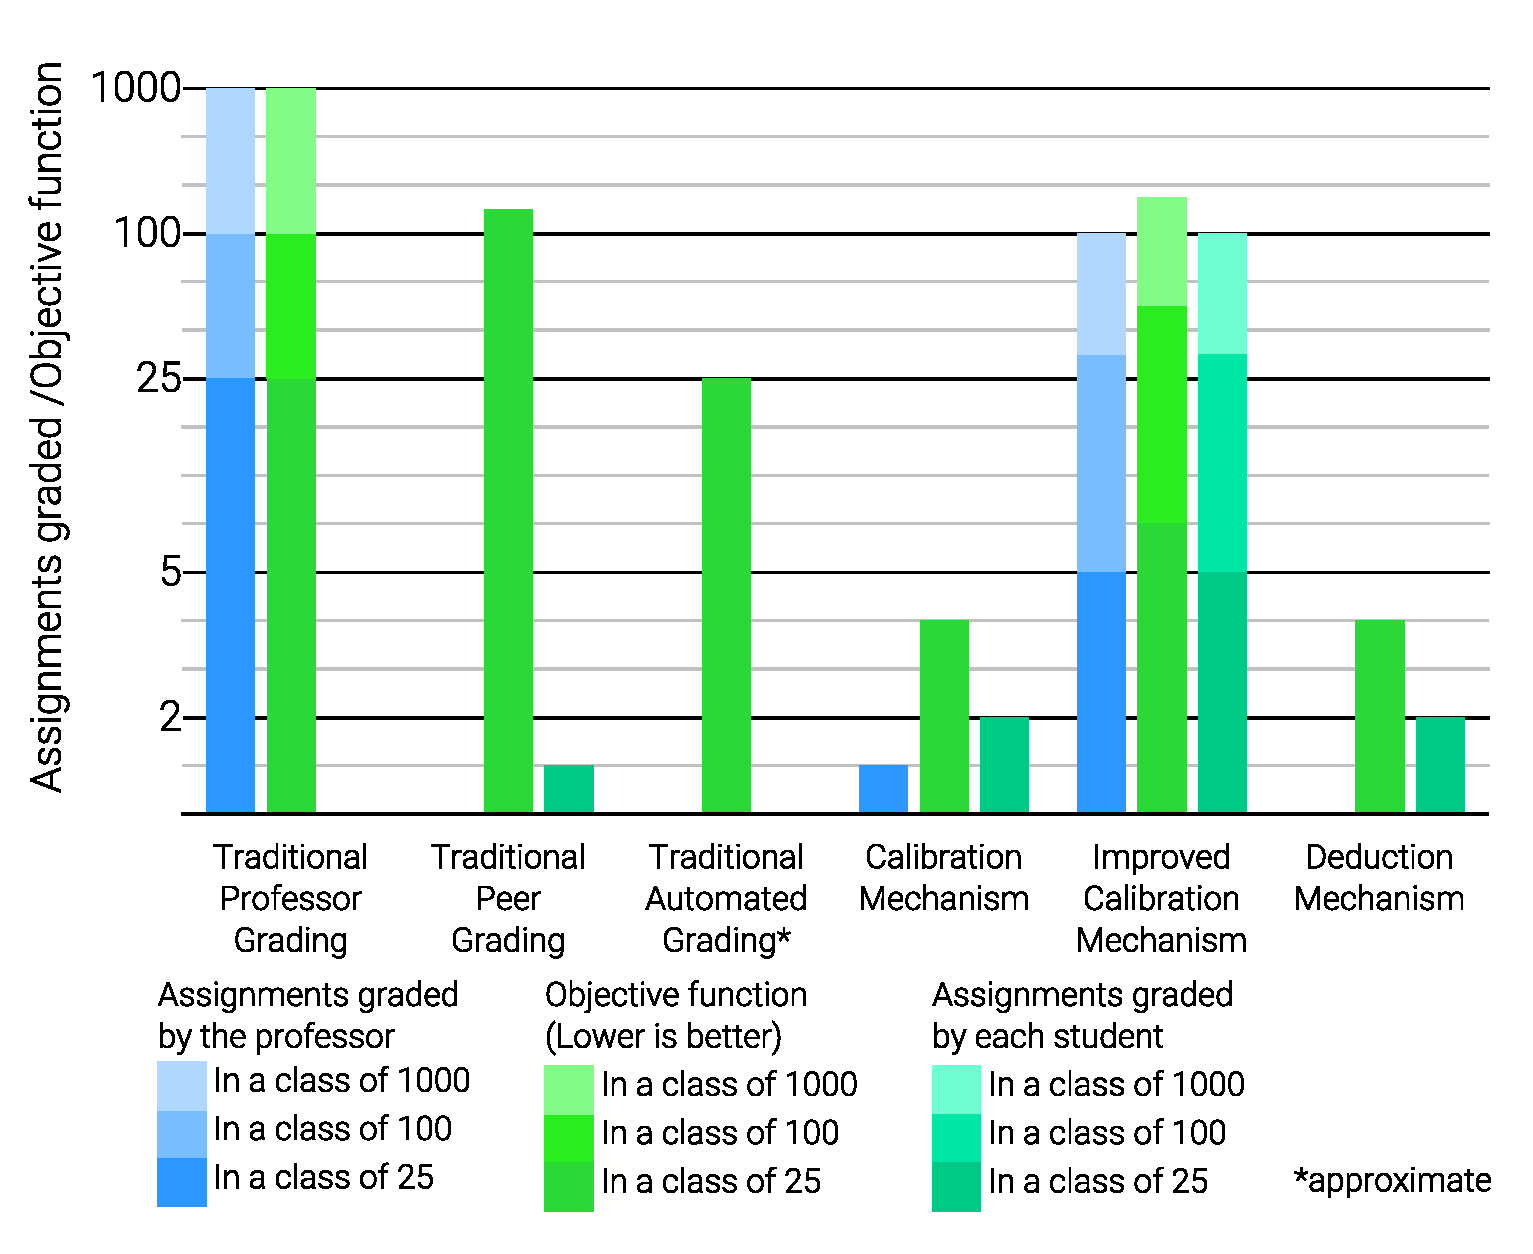
\includegraphics[width=\linewidth]{Comparison-Graph.eps}
  \caption{A comparison of mechanisms in terms of effectiveness and scalability.}
  \label{fig:comparison}
\end{figure}



% TODO: Accessibility

% TODO: Prep for Blind Review by removing authors

\section{Conclusion}
In this paper, a student model was first created - a set of assumptions that approximate the realistic behavior of students. Based on this model, various grading mechanisms were developed: Calibration, Improved Calibration, and Deduction. These mechanisms incentivize students to grade accurately and efficiently as proven by game theory. The Calibration mechanism was tested with a crowd-sourced experiment, showing that it could work in practice. The student model can easily be reused and improved upon by future researchers who wish to develop more efficient solutions to more realistic scenarios. Mechanism efficiency can be measured in terms of benchmark defined in this paper. The benchmark is a numerical score encompassing both the accuracy of grades and the effort spent by any one person. The inclusion of effort spent by any one person in the benchmark enables the grading system scalability to be taken into account. To the best of our knowledge, these are the first game-theory-based peer-grading mechanisms.

\section{Future Work}
The further improvement and development of mechanisms may involve adding more realistic assumptions to the student model, which in turn may require more complex mechanisms. For example, a more complex mechanism may be required to generate accurate grades from incompetent graders. Of course, more testing and validation of mechanisms with crowd-sourced experiments is necessary. Eventually, new mechanisms based off the student model or existing mechanisms could be implemented in commercial MOOCs such as EdX or Coursera.

\section{Acknowledgments}
We would like to thank MIT and the MIT PRIMES program for providing the research opportunity, as well as our parents for their support. Of course, none of this is possible without the original idea proposed by our advisor, Constantinos Daskalakis.

\balance
\bibliographystyle{acm-sigchi}
\bibliography{bibliography}

\end{document}